%!TEX root = ../main.tex
\setlength\belowcaptionskip{-1.5ex}

Στο κεφάλαιο \ref{ch:chap3} παρουσιάστηκε αναλυτικά η υλοποίηση της διπλωματικής εργασίας, απο την προεπεξεργασία και τροποποίηση των δεδομένων εως την παρουσίαση των αρχιτεκτονικών νευρωνικών δικτύων που χρησιμοποιήθηκαν. Σε αυτό το κεφάλαιο θα παρουσιαστούν τα αποτελέσματα και οι προβλέψεις των νευρωνικών δικτύων και θα πραγματοποιηθεί μια σύγκριση με αλλα υπάρχοντα μοντέλα πρόβλεψης αλληλεπιδράσεων πρωτεϊνών, αφού πρώτα ορισθούν όλες οι μετρικές αξιολόγησης των μοντέλων.


\section{Αποτελέσματα Εκπαίδευσης}

Προκειμένου να αξιολογήσουμε τα αποτελέσματα εκπαίδευσης, πρέπει να καθοριστεί το σύνολο των δεδομένων εκπαίδευσης με βάση το οποίο θα πραγματοποιηθεί η εκπαίδευση. Καθώς τα δεδομένα μας τροποποιήθηκαν από δύο αλγορίθμους, η λογική προσέγγιση θα ήταν η σύγκριση των αποτελεσμάτων εκπαίδευσης για τα δύο σύνολα και η επιλογή του συνόλου που αποδίδει καλύτερα. Ωστόσο, παρατηρώντας το περιεχόμενο των τιμών των δύο συνόλων ύστερα από την επεξεργασία, συμπεραίνουμε ότι έχουν παρόμοιες (σχεδόν πανομοιότυπες) εγγραφές, γεγονός που επιβεβαιώθηκε υπολογίζοντας την απόσταση \textit{Frobenius} των δύο μητρώων μέσω του τύπου: 

{\Large
$ dist(\textbf{A},\textbf{B}) =\sqrt{ \sum_{i=1}^{I}\sum_{j=1}^{J}( a_{ij} - b_{ij} )^2 } \approx 0$ }

\medskip
Επομένως, θα μπορούσαμε να επιλέξουμε ένα από τα δύο σύνολα εκπαίδευσης τυχαία για την εκπαίδευση/αξιολόγηση των μοντέλων μας. Ακόμη, παρατηρώντας τους χρόνους σύγκλισης των δύο αλγορίθμων, καταλήγουμε στη χρήση του συνόλου εκπαίδευσης που προέκυψε μέσω τανυστικής αποδόμησης για την εκπαίδευση των μοντέλων μας, καθώς η διαφορά στην ταχύτητα σύγκλισης καθιστά απαγορευτική την εκτέλεση της παραγοντοποίησης μητρώου μέσω SGD σε σχέση με την τανηστική αποδόμηση. 

\medskip
\begingroup
\centering
\newcommand\T{\rule{0pt}{3.0ex}} % Top strut
\newcommand\B{\rule[-2.0ex]{0pt}{0pt}} % Bottom strut
\begin{tabularx}{1\textwidth} { 
  | >{\centering\arraybackslash}X 
  | >{\centering\arraybackslash}X | }
 \hline
 \multicolumn{2}{|c|}{\textbf{Χρόνοι Σύγκλισης Μεθόδων}} \T\B \\
 \hline
 \textbf{Μέθοδος}\T\B & \textbf{Χρόνος (σε s)}\T\B \\
 \hline
 \textbf{Παραγοντοποίηση μητρώου μέσω SGD}\T\B & 1895.38\T\B \\
 \hline
 \textbf{CP αποδόμηση}\T\B & \textbf{26.04}\T\B \\
 \hline
\end{tabularx}
\captionof{table}{Χρόνοι σύγκλισης μεθόδων συμπλήρωσης μητρώων} 
\label{convtime}
\endgroup

\medskip
Όσον αφορά τα χρονικά αποτελέσματα της εκπαίδευσης, εμπειρικά παρατηρείται ότι η εκπαίδευση των πλήρως διασυνδεδεμένων επιπέδων ενός νευρωνικού δικτύου πραγματοποιείται πολύ πιο γρήγορα απ' ότι στην περίπτωση των συνελικτικών επιπέδων,ενώ τα συνελικτικά επίπεδα απαιτούν περισσότερη μνήμη για την αποθήκευση των ενδιάμεσων παραγώγων. Στην περίπτωσή μας, καθώς τα αποτελέσματα που παρουσιάζονται στη συνέχεια προέκυψαν από επικυρωμένη διασταύρωση (cross-validation), παρουσιάζονται οι χρόνοι για την εκπαίδευση μιας πτυχής (1 fold), με τα αποτελέσματα να εμφανίζονται στον πίνακα \ref{traintime}. Όπως παρατηρούμε,η εκπαίδευση του πλήρως διασυνδεδεμένου δικτύου χρειάστηκε \textbf{30} λιγότερες εποχές από αυτήν του συνελικτικού δικτύου, ωστόσο λόγω της γρηγορότερης εκτέλεσης των εποχών του συνελικτικού η εκπαίδευση του χρειάστηκε σχεδόν τον ίδιο χρόνο ($\approx 20$ λεπτά). Αξίζει να παρατηρηθεί επίσης ότι κάθε εποχή του συνελικτικού μοντέλου ήταν \textbf{1.33} φορές πιο γρήγορη από την αντίστοιχη του πλήρως διασυνδεδεμένου. Η συνθήκη σύγκλισης ήταν ίδια και για τα δύο μοντέλα και θεωρούσαμε σύγκλιση όταν δεν παρατηρούταν μεταβολή μικρότερη από $\delta = 2\times 10^{-4}$ στο \textit{σφάλμα επικύρωσης} (\textit{validation loss}) για ένα διάστημα 10 εποχών. 

\medskip
\begingroup
\centering
\newcommand\T{\rule{0pt}{3.0ex}} % Top strut
\newcommand\B{\rule[-2.0ex]{0pt}{0pt}} % Bottom strut
\begin{tabularx}{1\textwidth} { 
  | >{\centering\arraybackslash}X 
  | >{\centering\arraybackslash}X 
  | >{\centering\arraybackslash}X |}
 \hline
 \multicolumn{3}{|c|}{\textbf{Χρόνοι Σύγκλισης Μοντέλων}} \T\B \\
 \hline
 \textbf{Μοντέλο}\T\B & \textbf{Εποχές (ανά εποχή)} \T\B & \textbf{Χρόνος (σε s)}\T\B \\
 \hline
 \textbf{Πλήρως Διασυνδεδεμένο}\T\B & 75 (16.82s)\T\B & 1220.61 (20.3 λεπτά)\T\B \\
 \hline
 \textbf{Συνελικτικό}\T\B & 105 (12.61s)\T\B & 1225.28 (20.4 λεπτά)\T\B \\
 \hline
\end{tabularx}
\captionof{table}{Χρόνοι σύγκλισης νευρωνικών δικτύων} 
\label{traintime}
\endgroup

\newpage
\medskip
Παρακάτω, παρουσιάζονται οι γραφικές ακρίβειας και απωλειών των νευρωνικών δικτύων. Καθώς τα αποτελέσματα που παρουσιάζονται στη συνέχεια προέκυψαν από επικυρωμένη διασταύρωση (cross-validation), επιλέξαμε να αποτυπώσουμε τις απώλειες και την ακρίβεια ενδεικτικά για μια από τις 10 \textit{πτυχές} (folds). Φαίνεται από τις γραφικές παραστάσεις ότι το πλήρως διασυνδεδεμένο δίκτυο συγκλίνει αρκετά γρήγορα (75 εποχές) και μαθαίνει αρκετά γρήγορα το σύνολο εκπαίδευσης, κάτι που φαίνεται από την γρήγορη αύξηση της ακρίβειας και την πτώση των απωλειών. Ωστόσο, οι καμπύλες για τα δεδομένα επικύρωσης συγκλίνουν πολύ γρήγορα σε μια τιμή και στη συνέχεια παρουσιάζουν μια ταλαντωτική συμπεριφορά γύρω από αυτή, γεγονός που για να αποφευχθεί μας οδήγησε στην εκπαίδευση του πλήρως διασυνδεδεμένου μοντέλου με πολύ μικρό ρυθμό μάθησης ($= 0.00001$). Αυτό δείχνει την μεγάλη ευαισθησία του πλήρως διασυνδεδεμένου δικτύου, ενώ ταυτόχρονα δεν γενικεύει σε μεγάλο βαθμό. Από την άλλη, το συνελικτικό νευρωνικό δίκτυο απαιτεί περισσότερες εποχές για να συγκλινει (105 εποχές), ωστόσο συγκλίνει με πιο ομαλό τρόπο ενω δεν δείχνει να παρουσιάζει την έντονη ταλαντωτική συμπεριφορά του πλήρως διασυνδεδεμένου δικτύου, γι' αυτό και χρησιμοποιήθηκε μεγαλύτερη τιμή για τον ρυθμό μάθησης ($= 0.0001$).

\begin{figure}[H]
  \centering
  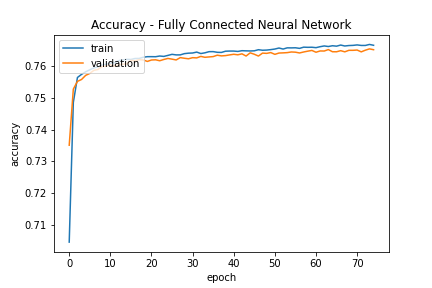
\includegraphics[width=1\textwidth]{images/DNNacc.png}
  \caption{Ακρίβεια πλήρως διασυνδεδεμένου νευρωνικού δικτύου}
  \label{fig:DNNacc}
\end{figure}

\begin{figure}[H]
  \centering
  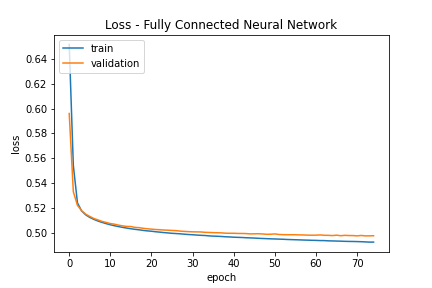
\includegraphics[width=1\textwidth]{images/DNNloss.png}
  \caption{Απώλειες πλήρως διασυνδεδεμένου νευρωνικού δικτύου}
  \label{fig:DNNloss}
\end{figure}

\begin{figure}[H]
  \centering
  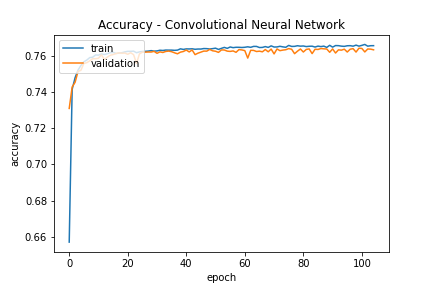
\includegraphics[width=1\textwidth]{images/CNNacc.png}
  \caption{Ακρίβεια συνελικτικού νευρωνικού δικτύου}
  \label{fig:CNNacc}
\end{figure}

\begin{figure}[H]
  \centering
  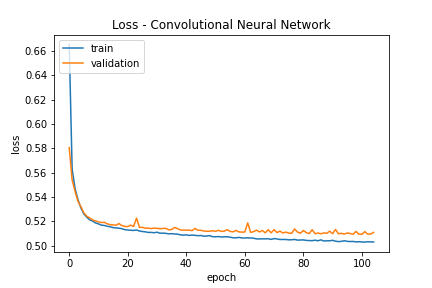
\includegraphics[width=1\textwidth]{images/CNNloss.png}
  \caption{Απώλειες συνελικτικού νευρωνικού δικτύου}
  \label{fig:CNNloss}
\end{figure}

Στη συνέχεια θα αναφερθούμε στις μετρικές που χρησιμοποιήθηκαν για την αξιολόγηση των μοντέλων μας. Αρχικά, η αντικειμενική συνάρτηση με βάση την οποία βελτιστοποιήθηκαν τα μοντέλα μας ήταν η \textit{απώλεια δυαδικής διασταυρωμένης εντροπίας} (\textit{binary crossentropy loss}).

{\noindent \Large
\begin{equation}
   J(w)= \frac{1}{m} \sum_{i=1}^{m}[ y_{i}*\log{\sigma(w^{\textit{T}}x_{i})} + (1-y_i)*\log{(1-\sigma(w^{\textit{T}}x_{i}))} ]
\end{equation}}

Για την αξιολόγηση της απόδοσης των μοντέλων και τη σύγκριση των αποτελεσμάτων χρησιμοποιήθηκαν οι ακόλουθες μετρικές:

\textit{Sensitivity}: Μετρική που εκφράζει την ποσότητα των θετικών περιπτώσεων που κατηγοριοποιούνται σωστά. Αποτελεί την σημαντικότερη μετρική όταν η αποφυγή των \textit{false negatives} έχει την ύψιστη σημασία.

\textit{Specificity}: Αντίστοιχη μετρική με το sensitivity, εκφράζει την ποσότητα των αρνητικών περιπτώσεων που κατηγοριοποιούνται σωστά, σημαντικό όταν μας απασχολούν τα \textit{false positives}.

\textit{Precision}: Μετρική που εκφράζει την πιθανότητα μιας θετικής κατηγοριοποίησης να είναι σωστή σε σχέση με όλες τις θετικές περιπτώσεις.

\textit{Accuracy}: Η πιο διαδεδομένη μετρική, εκφράζει την πιθανότητα μια κατηγοριοποίηση να είναι σωστή, ωστόσο δεν είναι πάντοτε αξιόπιστη στην περίπτωση δεδομένων που παρουσιάζουν \textit{ανισσοροπία} (\textit{imbalanced data sets}).

\textit{F1-score}: Αποτελεί τον αρμονικό μέσο των sensitivity και recall και αποτελεί ένα μέτρο αξιολόγησης της αποδοτικότητας ενός κατηγοριοποιητή, ωστόσο δεν λαμβάνει υπόψιν τις περιπτώσεις των \textit{true negatives}, εστιάζοντας κυρίως στις θετικές κατηγοριοποιήσεις.

\textit{MCC}: Γνωστή ως \textit{Matthew's Correlation Coefficient}, είναι ένα μέτρο συσχέτισης μεταξύ της πραγματικής τιμής και της πρόβλεψης. Λαμβάνει τιμές από $-1 - 1$, με το 0 να δηλώνει ότι οι προβλέψεις γίνονται τυχαία.

\medskip
\begingroup
\centering
\newcommand\T{\rule{0pt}{3.0ex}} % Top strut
\newcommand\B{\rule[-1.6ex]{0pt}{0pt}} % Bottom strut
\begin{tabularx}{1\textwidth} { 
  | >{\raggedright\arraybackslash}X 
   >{\centering\arraybackslash}X
   >{\raggedleft\arraybackslash}X | }
 \hline
 \multicolumn{3}{|c|}{\textbf{Μετρικές απόδοσης δυαδικής κατηγοριοποίησης}} \T\B \\
 \hline
 \textbf{Μετρική}\T\B & \textbf{Τύπος}\T\B & \textbf{Εύρος τιμών} \T\B \\
 \hline
 Sensitivity \T\B & {\Large$\frac{\textit{TP}}{\textit{TP+FN}}$ \T\B} & $[0,1]$\T\B \\
 \hline
 Specificity \T\B & {\Large$\frac{\textit{TN}}{\textit{TN+FP}}$ \T\B} & $[0,1]$\T\B \\
 \hline
 Precision \T\B & {\Large$\frac{\textit{TP}}{\textit{TP+FP}}$ \T\B} & $[0,1]$\T\B \\
 \hline
 Accuracy \T\B & {\Large$\frac{\textit{TP+TN}}{\textit{TP+TN+FP+FN}}$ \T\B} & $[0,1]$\T\B \\
 \hline
 F1 \T\B & {\Large$\frac{\textit{2TP}}{\textit{2TP+FP+FN}}$ \T\B} & $[0,1]$\T\B \\
 \hline
 MCC \T\B & {\Large $\frac{\textit{TP x TN - FP x FN}}{\sqrt{(\textit{TP}+\textit{FP}) (\textit{TP}+\textit{FN}) (\textit{TN}+\textit{FP}) (\textit{TN}+\textit{FN})}}$}\T\B & $[-1,1]$\T\B \\
 \hline
\end{tabularx}
\captionof{table}{Μετρικές απόδοσης δυαδικής κατηγοριοποίησης} 
\label{binarymetrics}
\endgroup

\medskip
Στον πίνακα \ref{binarymetrics} παρουσιάζονται οι μαθηματικοί τύποι που ορίζουν τις παραπάνω μετρικές. Ως \textit{true positive} (\textit{TP}) ορίζεται μια θετική περίπτωση που κατηγοριοποιείται ως θετική, ως \textit{false positive} (\textit{FP}) μια αρνητική περίπτωση που κατηγοριοποιείται ως θετική, ως \textit{true negative} (\textit{TN}) μια αρνητική περίπτωση που κατηγοριοποιείται ως αρνητική ενώ ως \textit{false negative} (\textit{FP}) μια αρνητική περίπτωση που κατηγοριοποιείται ως θετική.

\medskip
Εχοντας ορίσει τις μετρικές στον πίνακα \ref{binarymetrics}, προχωράμε στην εισαγωγή μερικών ακόμη εννοιών για την περαιτέρω κατανόηση των αποτελεσμάτων μας. Η πρώτη έννοια στην οποία θα αναφερθούμε είναι η \textit{καμπύλη AUC-ROC} (\textit{Area Under Curve - Reciever Operation Characteristics}). Η καμπύλη ROC αποτελεί μια μετρική που χρησιμοποιείται σε προβλήματα δυαδικής κατηγοριοποίησης προκειμένου να αξιολογηθεί η ποιότητα της εξόδου του κατηγοριοποιητή. Πρόκειται για μια καμπύλη πιθανότητας για διαφορετικές κατηγορίες, που εκφράζει την ικανότητα του μοντέλου να ξεχωρίσει τις δεδομένες κατηγορίες ως προς τις πιθανότητες πρόβλεψης. Στην εικόνα \ref{fig:ROC} φαίνεται μια τυπική καμπύλη ROC. Στον άξονα X υπάρχει ο ρυθμός \textit{False Positive}, δηλαδή την πιθανότητα μια αρνητική πρόβλεψη να είναι θετική, ενώ στον άξονα Y εχουμε τον ρυθμό \textit{True Positive}, δηλαδή την πιθανότητα μια θετική πρόβλεψη να είναι θετική. Εναλλακτικά, ο ρυθμός \textit{False Positive} αντιστοιχεί στην τιμή $1$-Specificity ενώ ο ρυθμός \textit{True Positive} αντιστοιχεί στην τιμή του Sensitivity.

\begin{figure}[H]
  \centering
  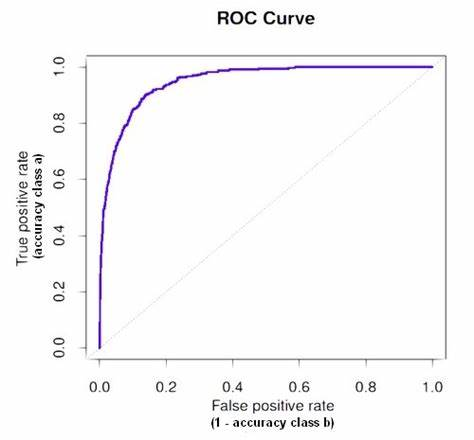
\includegraphics[width=1\textwidth]{images/ROC.jpg}
  \caption{Τυπική Καμπύλη ROC}
  \label{fig:ROC}
\end{figure}

\smallskip
Σχετικά με το περιεχόμενο της εικόνας \ref{fig:ROC}, ενα μοντέλο που προβλέπει τυχαία παρουσιάζει καμπύλη ROC που θα μοιάζει με την διαγώνια γκρι γραμμή και δεν έχει ικανότητα διάκρισης. Αντίθετα, όσο απομακρύνεται η καμπύλη από την διαγώνια γραμμή, τόσο καλύτερο είναι το μοντέλο στο να ξεχωρίζει τις θετικές περιπτώσεις από τις αρνητικές. Με βάση την παραπάνω καμπύλη, μπορούμε να εξάγουμε ορισμένες χρήσιμες μετρικές, όπως το σκορ \textit{AUC}. Οπως αναφέρει και το όνομα του, το AUC υπολογίζεται ως το εμβαδόν που βρίσκεται κάτω από την καμπύλη ROC και έχει αρκετές ερμηνείες. Συνοπτικά, είναι "η πιθανότητα ο κατηγοριοποιητής να κατατάξει ένα τυχαίο θετικό δείγμα υψηλότερα από ένα τυχαίο αρνητικό δείγμα" \cite{Hand2009MeasuringCP}. Το σκόρ AUC για έναν κατηγοριοποιητή που κάνει τυχαίες προβλέψεις (εμβαδόν κάτω από την γκρι διαγώνιο) θα είναι $0.5$, ενώ όσο αυξάνεται πλησιάζοντας την μονάδα δηλώνει και καλύτερη ικανότητα πρόβλεψης. Παρακάτω παρατίθενται οι καμπύλες AUC-ROC για κάθε μοντέλο που αναπτύξαμε, με την επιπλέον προσθήκη όπου θεωρούμε διαδοχικά κάθε κατηγορία ως την "θετική" κατηγορία.

\begin{figure}[H]
  \centering
  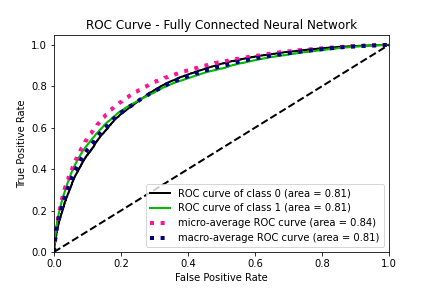
\includegraphics[width=1\textwidth]{images/DNNROC.png}
  \caption{Καμπύλη ROC πλήρως διασυνδεδεμένου νευρωνικού δικτύου}
  \label{fig:DNNROC}
\end{figure}

\begin{figure}[H]
  \centering
  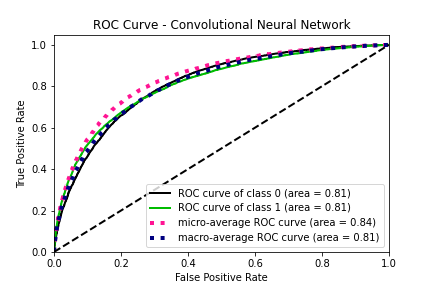
\includegraphics[width=1\textwidth]{images/CNNROC.png}
  \caption{Καμπύλη ROC συνελικτικού νευρωνικού δικτύου}
  \label{fig:CNNROC}
\end{figure}

Από τα αποτελέσματα παρατηρούμε ότι και οι δύο αρχιτεκτονικές παρέχουν αρκετά ικανοποιητικά αποτελέσματα όσον αφορά τις προβλέψεις. Συγκεκριμένα, και για τις δύο αρχιτεκτονικές υπολογίζουμε: \newline$AUC_{DNN} = 0.8148$ και $AUC_{CNN} = 0.8121$. Οι τιμές βρίσκονται αρκετά κοντά μεταξύ τους για να μπορούμε να ξεχωρίσουμε κάποια αρχιτεκτονική,απλώς παρατηρούμε ότι η πλήρως διασυνδεδεμένη αρχιτεκτονική αποδίδει ελαφρώς καλύτερα από την συνελικτική όσον αφορά τη συγκεκριμένη μετρική.

Άλλη μια γραφική που μας βοηθάει στην κατανόηση της αποδοτικότητας των μοντέλων μας είναι η \textit{καμπύλη ακρίβειας ανάκλησης} (\textit{Precision Recall curve}). Η διαφορά με την καμπύλη ROC έγκειται στο γεγονός ότι η καμπύλη ακρίβειας ανάκλησης εστιάζει στην κατηγορία που ορίζεται ως κατηγορία μειονότητας, δεν λαμβάνει υπόψιν τις αρνητικές κατηγοριοποιήσεις και μας παρέχει χρήσιμη πληροφορία στην περίπτωση που δουλεύουμε με \textit{ανισόρροπα}(\textit{imbalanced}) σύνολα εκπαίδευσης. Στον άξονα Y βρίσκεται το precision, που εκφράζει την πιθανότητα μιας θετικής σωστής κατηγοριοποίησης ως προς το σύνολο των θετικών περιπτώσεων, ενώ στον άξονα Χ το recall, που εκφράζει την πιθανότητα μιας θετικής κατηγοριοποίησης ως προς τον αριθμό των πιθανών θετικών κατηγοριοποιήσεων που θα μπορούσαν να συμβούν. Είναι επιθυμητό τα μοντέλα μας να έχουν ταυτόχρονα υψηλή ακρίβεια και υψηλή ανάκληση, ωστόσο στην πραγματικότητα υπάρχει ενα trade-off μεταξύ των δυο.

\begin{figure}[H]
  \centering
  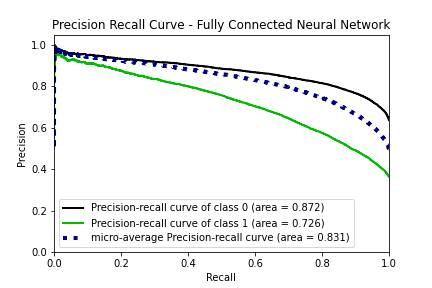
\includegraphics[width=1\textwidth]{images/DNNPRC.png}
  \caption{Καμπύλη Precision Recall πλήρως διασυνδεδεμένου νευρωνικού δικτύου}
  \label{fig:DNNPRC}
\end{figure}

\begin{figure}[H]
  \centering
  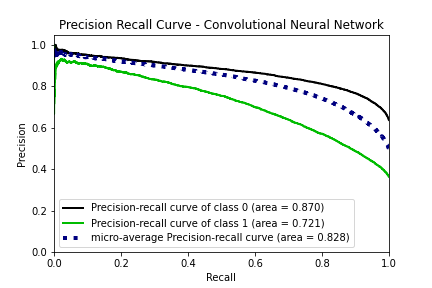
\includegraphics[width=1\textwidth]{images/CNNPRC.png}
  \caption{Καμπύλη Precision Recall συνελικτικού νευρωνικού δικτύου}
  \label{fig:CNNPRC}
\end{figure}
Παρατηρούμε ότι και στην περίπτωση της καμπύλης ακρίβειας-ανάκλησης, το πλήρως διασυνδεδεμένο νευρωνικό δίκτυο έχει οριακά καλύτερα αποτελέσματα από το συνελικτικό νευρωνικό δίκτυο. Στην περίπτωσή μας, η καμπύλες που μας απασχολούν είναι κυρίως οι καμπύλες που αφορούν την κατηγορίας 1, δηλαδή αυτές που ορίζουν ως θετική περίπτωση την ύπαρξη αλληλεπίδρασης. 

Στα αποτελέσματα της δημοσίευσης \cite{Northey2017} με την οποία συγκρίνουμε τα αποτελέσματά μας, λόγω της ύπαρξης \textit{NaN} τιμών στα χαρακτηριστικά του αρχικού συνόλου δεδομένων (ιδίως στα χαρακτηριστικά \textit{Conservation Scores}), παρατίθενται από τους συγγραφείς της δημοσίευσης τα αποτελέσματα για διαφορετικές περιπτώσεις εγγραφών. Στον παρακάτω πίνακα για τα αποτελέσματα των νευρωνικών δικτύων και των random forests επιλέχθηκαν τα αποτελέσματα όπου λαμβάνονται υπόψιν όλα τα χαρακτηριστικά. Στην περίπτωση που οι τιμές των χαρακτηριστικών είναι μη-έγκυρες, για τα νευρωνικά δίκτυα επιλέχθηκε μια τιμή που βασίζεται στον μέσο όρο της κατανομής των δεδομένων, ενώ για τα random forests χρησιμοποιήθηκε η μέθοδος \textit{fractional instances}, κατά την οποία εγγραφές που περιέχουν ελλιπείς τιμές διαιρούνται σε πολλαπλές τιμές με διαφορετικά βάρη.

\medskip
\begingroup
\centering
\newcommand\T{\rule{0pt}{3.0ex}} % Top strut
\newcommand\B{\rule[-1.6ex]{0pt}{0pt}} % Bottom strut
\begin{tabularx}{1\textwidth} { 
  |>{\raggedright\arraybackslash}X 
   >{\centering\arraybackslash}X
   >{\centering\arraybackslash}X
   >{\centering\arraybackslash}X
   >{\centering\arraybackslash}X
   >{\centering\arraybackslash}X
   >{\centering\arraybackslash}X | }
 \hline
 \multicolumn{7}{|c|}{\textbf{Σύγκριση μεθόδων}} \T\B \\
 \hline
 \textbf{Method} \T\B & \textbf{ACC}\T\B & \textbf{PREC} \T\B & \textbf{SPEC} \T\B & \textbf{SENS} \T\B & \textbf{F} \T\B & \textbf{MCC} \T\B \\
 \hline
 Neural Network \cite{Northey2017}  \T\B & $0.735$ \T\B & $0.653$ \T\B & $0.892$ \T\B & $0.415$ \T\B & $0.507$ \T\B & $0.355$ \T\B \\
 \hline
 Random Forest \cite{Northey2017} \T\B & \textbf{0.760} \T\B & $0.679$ \T\B & \textbf{0.906} \T\B & $0.439$ \T\B & $0.533$ \T\B & $0.398$ \T\B \\
 \hline
 CP + Fully Connected NN \T\B & $0.756$ \T\B & $0.756$ \T\B & $0.756$ \T\B & $0.756$ \T\B & $0.756$ \T\B & $0.512$ \T\B \\
 \hline
 CP + Convolu\-tional NN \T\B & $0.758$ \T\B & \textbf{0.758} \T\B & $0.758$ \T\B & \textbf{0.758} \T\B & \textbf{0.758} \T\B & \textbf{0.516} \T\B \\
 \hline
\end{tabularx}
\captionof{table}{Αποτελέσματα - Σύγκριση Μεθόδων} 
\label{binarymetrics}
\endgroup

\medskip
Τα παραπάνω αποτελέσματα αποδεικνύουν την βελτίωση της απόδοσης του κατηγοριοποιητή μέσω της συμπλήρωσης των ελλειπών τιμών και της χρήσης νευρωνικών δικτύων. Ειδικότερα, λαμβάνοντας υπόψιν τα αποτελέσματα του καλύτερου μοντέλου μας (αποδόμηση τανυστών και συνελικτική δομή νευρωνικών δικτύων), ενώ η απόδοση των νευρωνικών δικτύων που αναπτύξαμε είναι παρόμοια με αυτή της δημοσίευσης \cite{Northey2017}, η σωστή κατηγοριοποίηση των κομματιών επιφανείας (αύξηση του sensitivity κατά \textbf{72.66}$\%$ σε σχέση με τα random forests και κατά \textbf{82.65}$\%$ σε σχέση με την αρχιτεκτονική νευρωνικών δικτύων) καθώς και η συνολική αποδοτικότητα του κατηγοριοποιητή μας είναι σημαντικά βελτιωμένη. Χρησιμοποιώντας τον MCC ως κύρια μετρική αξιολόγησης, όπως πραγματοποιείται και στην δημοσίευση των Northey et al. και καθώς θεωρείται η καλύτερη μετρική αξιολόγησης ενός δυαδικού κατηγοριοποιητή σε θέματα υπολογιστικής βιολογίας, πετύχαμε αύξηση κατά \textbf{29.65}$\%$ σε σχέση με την αρχιτεκτονική των random forests και κατά \textbf{45.35}$\%$ σε σχέση με την αρχιτεκτονική νευρωνικών δικτύων \cite{Northey2017}. 

\newpage
\section{Μελλοντικές Εξελίξεις}

Στην ενότητα αυτή παρουσιάζονται διάφορες ιδέες σχετικά με την επέκταση της παρούσας διπλωματικής. Αρχικά, η πιο απλή διαδικασία για την βελτίωση των αποτελεσμάτων προέρχεται από την εκπαίδευση των μοντέλων μηχανικής μάθησης με ολοένα και περισσότερα δεδομένα και η αξιολόγηση τους σε ανεξάρτητα σύνολα αξιολόγησης, επομένως ως πρώτο βήμα θα μπορούσαν να εξαχθούν νέα δεδομένα από την πρωτεϊνική βάση δεδομένων PDB και να κατασκευαστούν νέα σύνολα δεδομένων εκπαίδευσης και αξιολόγησης με πιο σύγχρονα δεδομένα.

\medskip
Παράλληλα, όσον αφορά το σύνολο των δεδομένων εκπαίδευσης, θα μπορούσαν να προστεθούν περισσότερα χαρακτηριστικά, τόσο δομικά όσο και ακολουθιακά, για την εξαγωγή επιπλέον πληροφορίας σχετικά με τις αλληλεπιδράσεις μεταξύ πρωτεϊνών. Μερικά χαρακτηριστικά που παρουσιάζουν θετικά αποτελέσματα είναι οι \textit{φυσικοχημικές} ιδιότητες των αμινοξέων (\textit{physicochemical properties of amino acids}) \cite{Xie2020} και το \textit{σκορ αταξίας} (\textit{disorder score}) \cite{Li2012}.

\medskip
Όσον αφορά την προεπεξεργασία των δεδομένων, οι μέθοδοι συμπλήρωσης μητρώου λειτουργούν ιδανικά με μεγάλες δομές δεδομένων, γεγονός που δεν συμβαίνει στην περίπτωσή μας όπου έχουμε μόνο 8 χαρακτηριστικά. Ωστόσο, η ήδη υπάρχουσα απόδοση των αλγορίθμων θα μπορούσε να συγκριθεί με διαφορετικές μεθόδους. Μια σκέψη περιλαμβάνει την αξιολόγηση της τανηστικής αποδόμησης με πειραματισμους όσον αφορά την τιμή των $\beta_k$ \ref{beta} κατά την εφαρμογή των μεθόδων μη γραμμικής συζηγούς παραγώγου (ncg). Αντίστοιχα, θα μπορούσε να ελεγχθεί η αύξηση της ταχύτητας σύγκλισης του αλγορίθμου παραγοντοποίησης μητρώου μέσω SGD εφόσον υλοποιηθεί με κατανεμημένο τρόπο μέσω της τροποποιημένης μορφής του SGD που ονομάζεται \textit{Stratified Stochastic Gradient Descent} (\textit{SSGD}) \cite{Gemulla2011}.